\apendice{Manual de especificación de diseño}

A continuación, se presenta el diseño técnico del sistema de pulsioximetría desarrollado, incluyendo los esquemas eléctricos más relevantes y los diagramas de bloques de los algoritmos utilizados, con el objetivo de dejar documentada la arquitectura general tanto a nivel de hardware como de procesamiento de señal. 

Dado que el desarrollo se ha realizado a partir de material previamente existente, se ha incluido una sección que contextualiza el estado del sistema antes del inicio del trabajo, detallando los recursos existentes proporcionados por el equipo de \textit{In$^3$ator} sobre los que se ha construido esta implementación.

\section{Punto de partida}

El presente trabajo parte de una base sólida ya desarrollada por el equipo de la ONG Medicina Abierta al Mundo, responsable del diseño, fabricación y distribución de la incubadora de bajo coste \textit{In$^3$ator} (figura \ref{fig:in3ator23}). 

Esta incubadora, que ha sido puesta en funcionamiento en países con recursos limitados, cuenta con un sistema electrónico y de control completamente operativo, cuyo diseño de hardware y firmware cubre funciones esenciales como la regulación de temperatura, humedad, ventilación, fototerapia y alarmas de seguridad.

\begin{figure}[H]
    \centering
    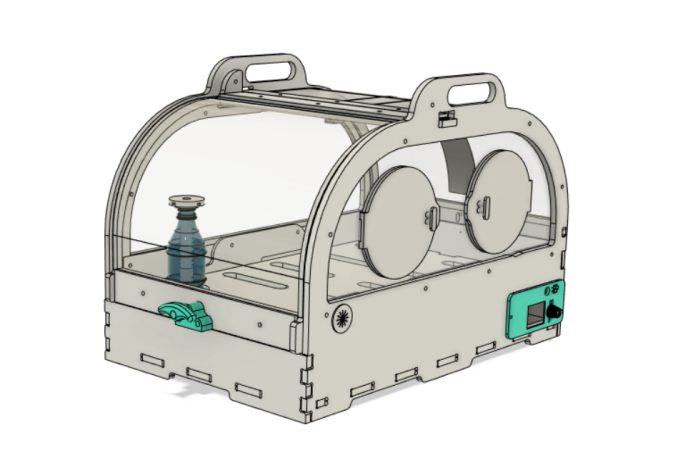
\includegraphics[width=0.75\linewidth]{img/in3ator23.png}
    \caption{Diseño 3D de la incubadora neonatal \textit{In$^3$ator} version 2.1. Fuente: \cite{in3ator2023manual}.}
    \label{fig:in3ator23}
\end{figure}

Actualmente, las incubadoras distribuidas por la ONG no cuentan con funcionalidad de pulsioximetría integrada. Sin embargo, con el objetivo de investigar su posible implementación, el equipo de \textit{In$^3$ator} incorporó de forma experimental esta funcionalidad en el hardware (figura \ref{fig:PCB2}) de un prototipo. Este sistema nos fue cedido para el desarrollo y validación del algoritmo correspondiente. La placa electrónica ya disponía de un sistema de adquisición basado en el AFE4490, así como de una interfaz con el microcontrolador ESP32. 

\begin{figure}[H]
    \centering
    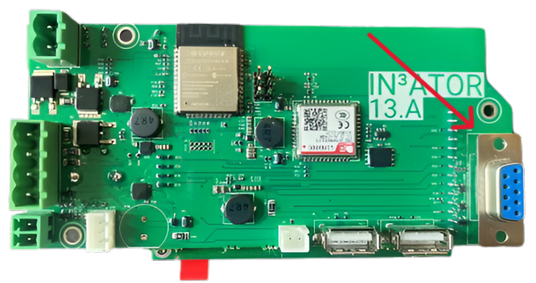
\includegraphics[width=0.75\linewidth]{img/PCB2.png}
    \caption{Placa electrónica modificada con la funcionalidad de pulsioximetría integrada. Fuente: \textit{Elaboración propia}.}
    \label{fig:PCB2}
\end{figure}

El firmware general del sistema estaba también desarrollado, con una estructura que permitía incorporar nuevas funciones. Dentro de este contexto, mi trabajo se ha centrado en el archivo \texttt{SPO2.cpp} (\ref{fig:firmware}), donde he implementado, por una parte, la función que extraía los datos crudos del sensor para poder estudiar los procedimientos por separado; y por otra, el algoritmo de estimación de frecuencia cardíaca y saturación de oxígeno a partir de las señales obtenidas por el sensor óptico en tiempo real.

\begin{figure}[H]
    \centering
    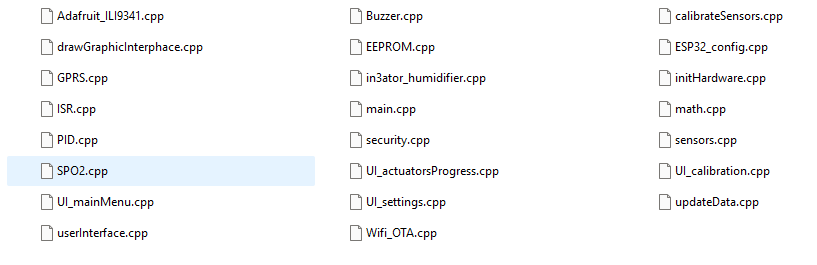
\includegraphics[width=1\linewidth]{img/firmware.png}
    \caption{Estructura de archivos del directorio \texttt{src/}del firmware original. \textit{Elaboración propia}.}
    \label{fig:firmware}
\end{figure}

Para desarrollar estos algoritmos, se realizó primero un estudio experimental en Python a través de Jupyter Notebooks, partiendo desde cero, basándome en artículos científicos y documentos técnicos, como los proporcionados por fabricantes de sensores comerciales (por ejemplo, OB1203). A partir de estos análisis, se seleccionaron los métodos más adecuados para su implementación en el entorno embebido del ESP32.

En cuanto a la integración hardware, no fue necesario modificar la placa, ya que era completamente funcional. Mi labor consistió en aprender a conectarla correctamente, instalar los drivers necesarios y adquirir pulsioxímetros comerciales como referencia externa para validar los resultados obtenidos por el sistema. Para ello, se nos proporcionaron los planos correspondientes a la estructura electrónica de la placa donde se podía observar con detalle la disposición de los componentes relevantes para la funcionalidad de pulsioximetría. Estos planos se analizan a continuación con el objetivo de contextualizar el entorno hardware sobre el que se desarrolló este proyecto.

\newpage

\section{Planos}

En esta sección se recogen los esquemas eléctricos relacionados con el subsistema de pulsioximetría implementado en este trabajo. Los planos han sido extraídos de los esquemáticos completos \footnote{Accesibles desde GitHub, dentro del directorio principal de \texttt{Documentación de referencia}} proporcionados por el equipo de desarrollo del proyecto \textit{In$^3$ator}, centrándose exclusivamente en los componentes que intervienen en la adquisición y transmisión de las señales fotopletismográficas.

La implementación se basa en tres bloques:
\begin{itemize}
    \item El \textbf{AFE4490}, un circuito especializado que capta y digitaliza la señal óptica procedente del sensor de pulsioximetría.
    \item El \textbf{sistema de alimentación}, que permite el funcionamiento autónomo mediante batería y gestiona la distribución de voltajes adecuados a cada componente.
    \item El \textbf{microcontrolador ESP32}, que ejecuta el firmware encargado de controlar el sensor, procesar las señales y enviar los datos.
\end{itemize}

A continuación se muestran los esquemas correspondientes, cada uno acompañado de una breve descripción técnica que resume su funcionalidad dentro del sistema.
\subsection{Circuito de adquisición AFE4490}

Este circuito es el encargado de recibir la se\~nal \'optica captada por el sensor (LED y fotodiodo), amplificarla, filtrarla y convertirla a formato digital. Aunque el esquema incluye muchos componentes, lo m\'as relevante para este proyecto es identificar el chip AFE4490, las entradas de se\~nal, y las conexiones SPI que permiten que el microcontrolador reciba los datos digitalizados.

\begin{figure}[H]
\centering
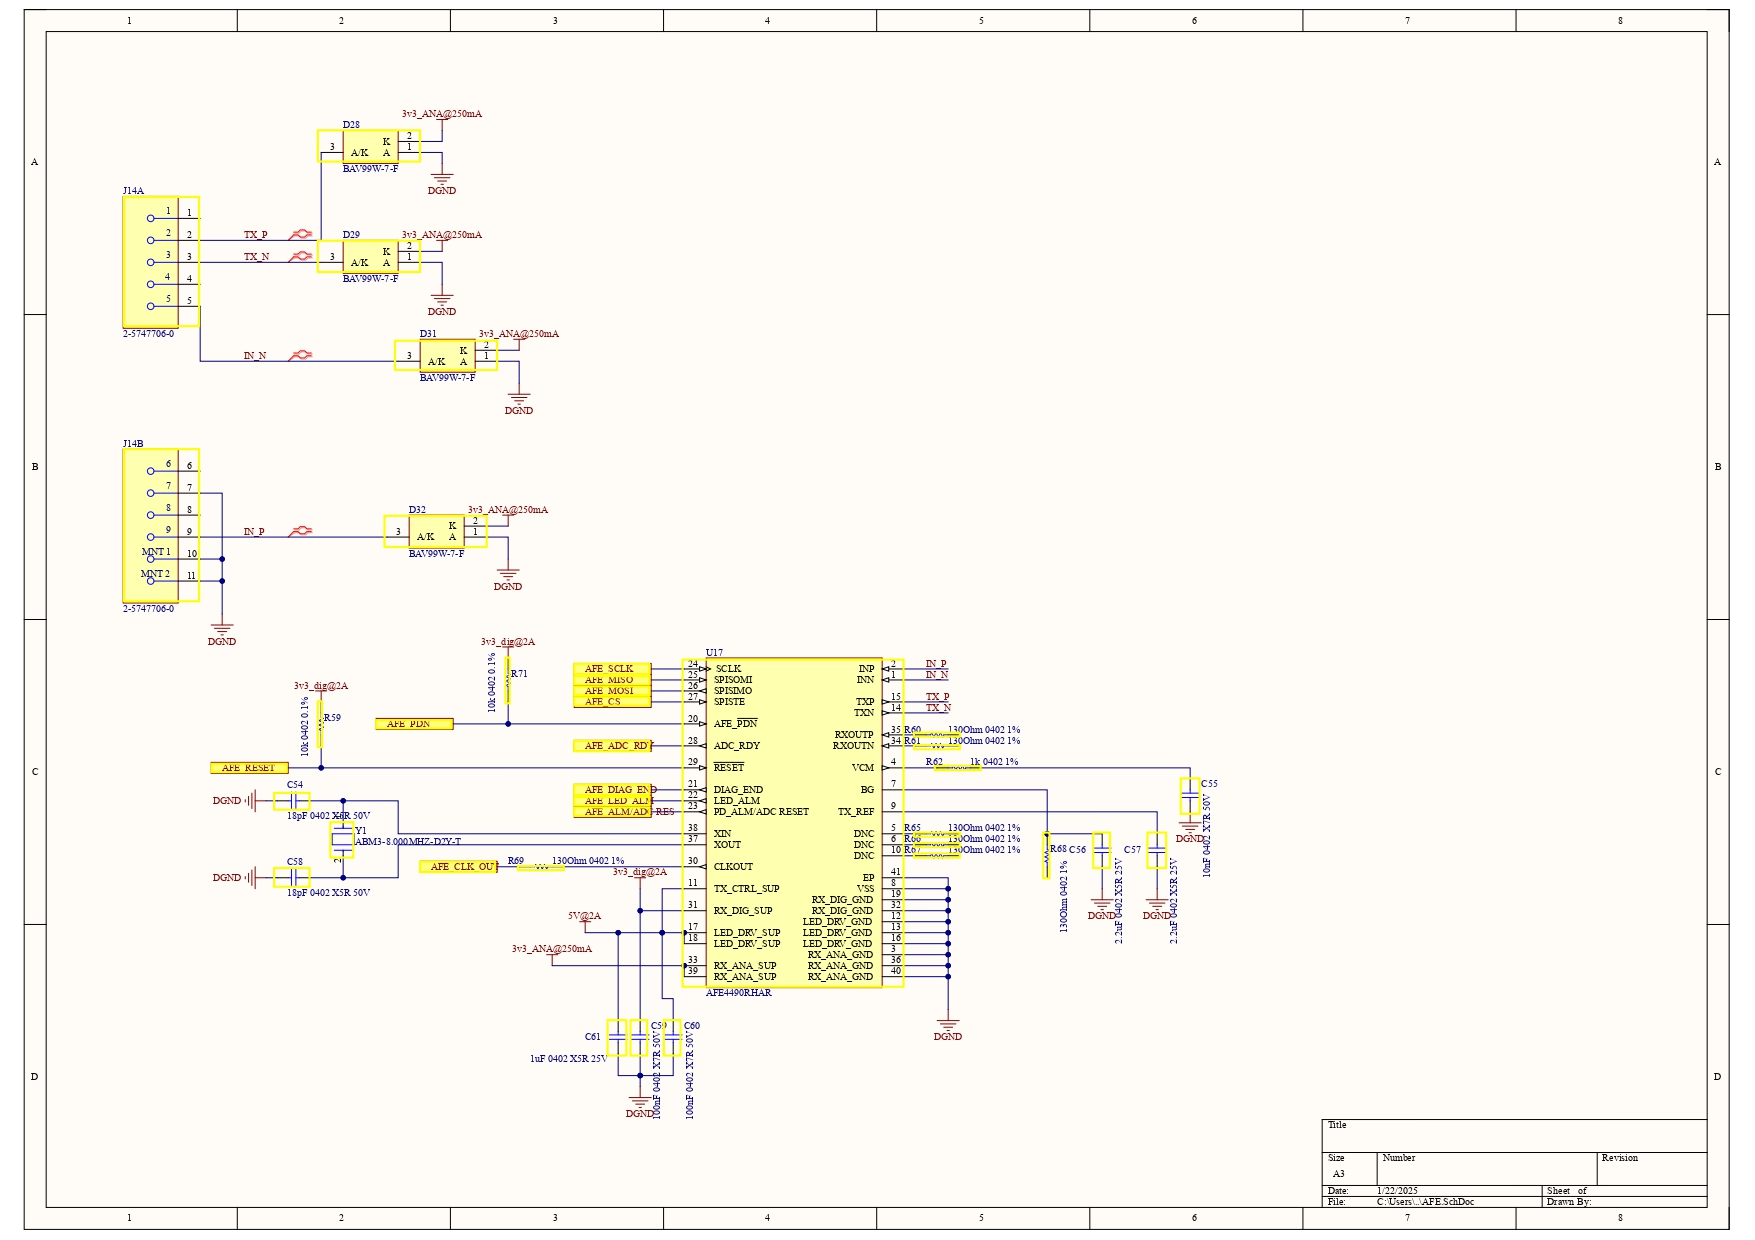
\includegraphics[width=1\textwidth]{img/AFE.jpg}
\caption{Esquema eléctrico del circuito AFE4490, incluyendo alimentación analógica y digital, señales de control y líneas SPI de comunicación con el microcontrolador. Extraído del fichero \texttt{AFE.SchDoc}. Fuente: \href{https://medicalopenworld.org/}{MedicalOpenWorld}.}
\end{figure}

Físicamente, en el hardware, el AFE4490 se encuentra en el reverso de la PCB, es de muy pequeño tamaño y tiene este aspecto:

\begin{figure}[H]
    \centering
    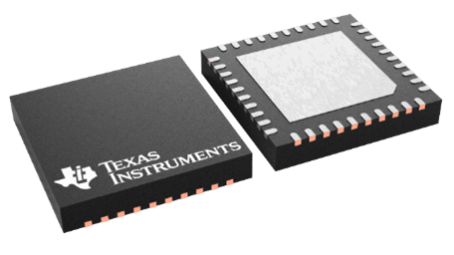
\includegraphics[width=0.5\linewidth]{img/AFE.png}
    \caption{Extremo frontal analógico integrado (AFE) para pulsioxímetros. Imagen referencial del componente físico AFE4490. Fuente: \href{https://www.ti.com/product/es-mx/AFE4490/part-details/AFE4490RHAT}{TexasInstruments.}}
    \label{fig:AFE2}
\end{figure}


\subsection{Gestión de alimentación y carga de batería}

Este plano muestra la parte del circuito que permite alimentar todo el sistema a partir de una batería de 12V. Es importante fijarse en los reguladores de tensión que convierten esa entrada a los 3.3V necesarios para el AFE4490 y el ESP32. 


\begin{figure}[H]
    \centering
    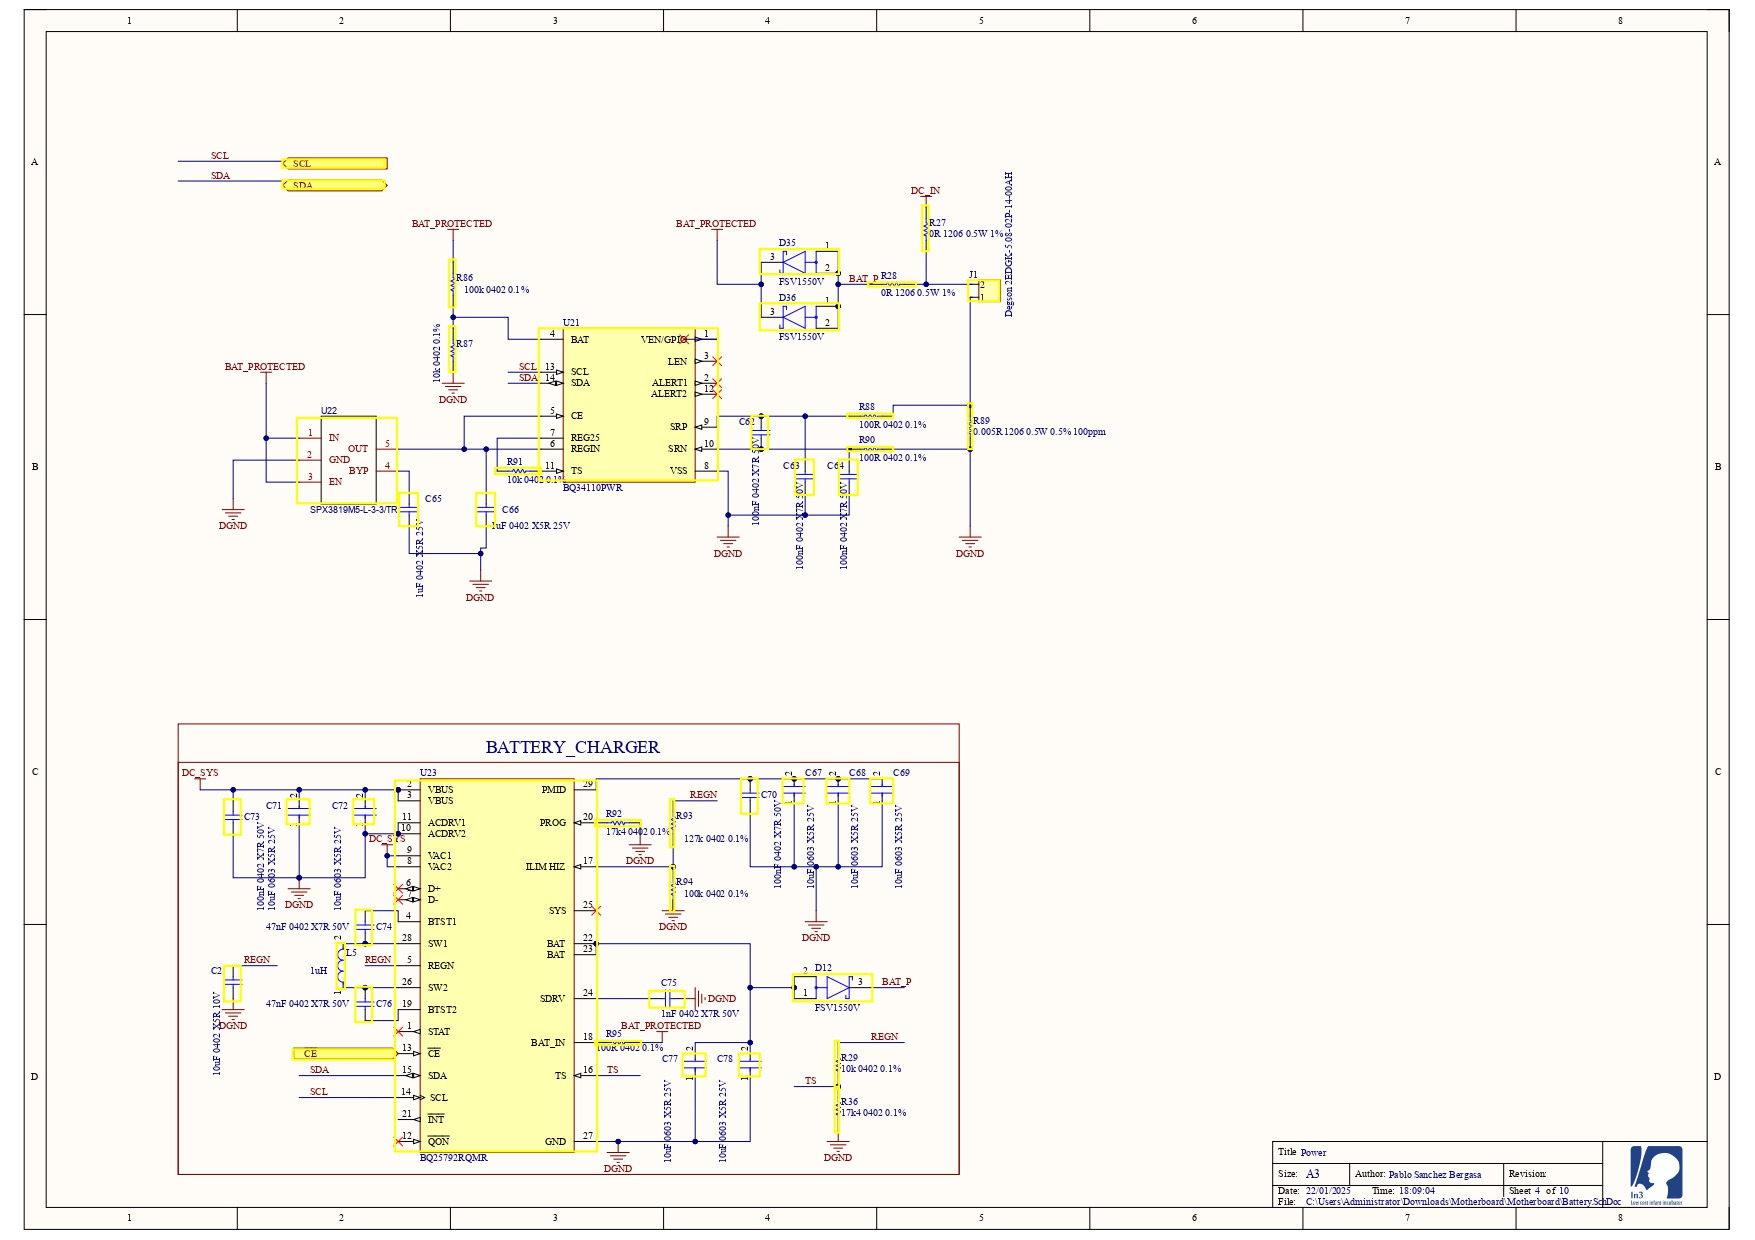
\includegraphics[width=1\linewidth]{img/Battery.jpg}
    \caption{Esquema de alimentación del sistema, donde se aprecia la fuente principal de 5V, la conversión a 3.3V digital y analógico, y la distribución de potencia hacia el AFE y el microcontrolador. Extraído del fichero \texttt{Power\_Input.SchDoc}. Fuente: \href{https://medicalopenworld.org/}{MedicalOpenWorld}}
    \label{fig:Battery}
\end{figure}

\subsection{Microcontrolador ESP32}

Este es el cerebro del sistema. En el plano se puede localizar el microcontrolador ESP32-WROOM-32, sus pines de entrada/salida y las conexiones hacia el AFE4490 mediante el bus SPI. Lo importante es fijarse en la relación entre los pines marcados como MOSI, MISO, SCK y CS, y las señales que se intercambian con el AFE.


\begin{figure}[H]
\centering
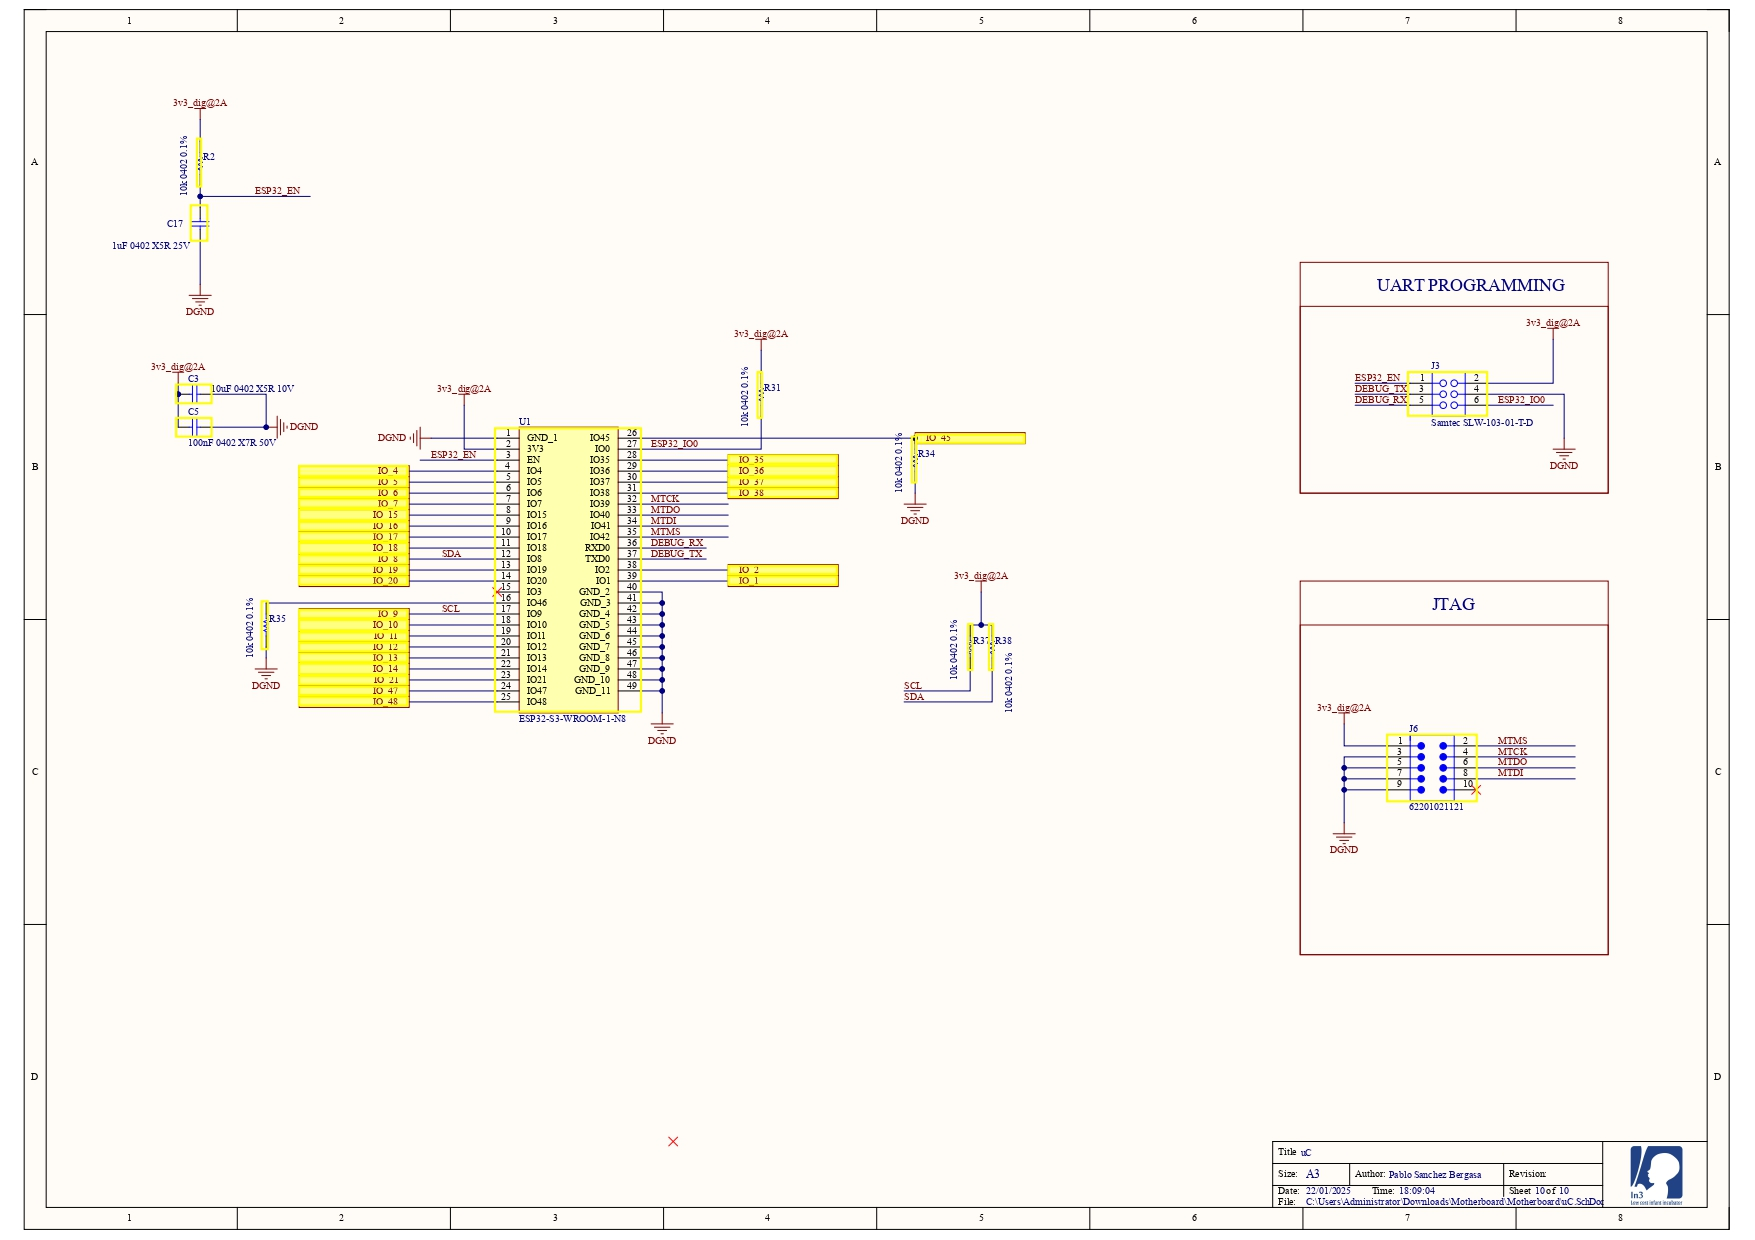
\includegraphics[width=1\textwidth]{img/Uc.jpg}
\caption{Plano del microcontrolador ESP32-WROOM-32. Extraído del fichero \texttt{Uc.SchDoc} Fuente: \href{https://medicalopenworld.org/}{MedicalOpenWorld} }
\end{figure}


Estos esquemas permitieron visualizar al inicio del proyecto cómo se integran a nivel de hardware los principales componentes implicados en la adquisición de señales PPG, así como su conexión con el microcontrolador que ejecuta el firmware desarrollado. 


\section{Diseño arquitectónico}

Dado que este proyecto no corresponde a una aplicación móvil o de escritorio, basada en objetos, sino a un sistema embebido de adquisición y procesamiento de señales biomédicas, se ha optado por no incluir diagramas clásicos como los de clases, secuencia o despliegue.

En su lugar, esta sección incluye diagramas de bloques que describen el comportamiento de los algoritmos implementados para la estimación de frecuencia cardíaca y SpO$_2$, basados en las señales adquiridas por el sensor. Estos diagramas reflejan las etapas de procesamiento y el flujo de datos desde la adquisición hasta el cálculo final de los parámetros fisiológicos.

\subsection{Algoritmos de estimación de la frecuencia cardíaca}

Los algoritmos que se muestran a continuación se han aplicado sobre los archivos CSV generados a partir del sistema de adquisición de datos descrito en el Anexo D y en la metodología de la memoria.

A continuación, se presentan los diagramas de los dos métodos que ofrecieron mejores resultados para la estimación de la frecuencia cardíaca, basados ambos en la detección de picos de la señal PPG, pero con enfoques distintos de preprocesamiento.

\subsubsection{Algoritmo 1: Filtro de media móvil}

El código correspondiente a este algoritmo se encuentra en el notebook \texttt{spo2.ipynb}. Los pasos seguidos se representan en la figura \ref{fig: diagrama1}.

\begin{figure}[H]
    \centering
    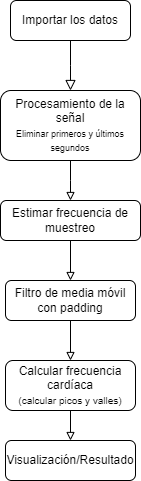
\includegraphics[scale = 0.65]{img/medias_moviles.png}
    \caption{Diagrama de bloques del algoritmo de frecuencia cardíaca basado en media móvil. \textit{Elaboración propia.}}
    \label{fig: diagrama1}
\end{figure}

\subsubsection{Algoritmo 2: Filtro paso bajo y detección con SciPy}

El código correspondiente a este algoritmo se encuentra en el notebook \texttt{pulsi\_comercial.ipynb}.El proceso se muestra en la figura \ref{fig: paso_bajo2}.

\begin{figure}[H]
    \centering
    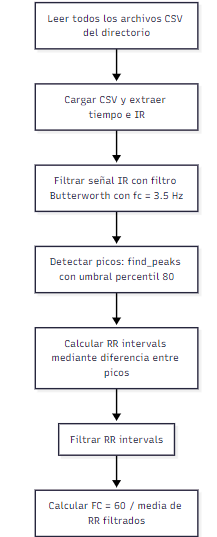
\includegraphics[scale = 0.65]{img/paso_bajo.png}
    \caption{Diagrama de bloques del algoritmo de frecuencia cardíaca con filtrado paso-bajo y detección por picos.\textit{Elaboración propia.}}
    \label{fig: paso_bajo2}
\end{figure}

Como se defendió en la metodología de la memoria teórica, se escogió el método que utiliza el preprocesamiento con media móvil + mediana. La elección entre uno u otro dependió del nivel de optimización y el coste computacional.

\subsection{Algoritmos de estimación de la saturación de oxígeno}

Para el cálculo de la SpO$_2$, inicialmente se desarrollaron versiones sencillas que aplicaban el cálculo clásico del ratio con aproximaciones teóricas o coeficientes fijos. Sin embargo, los mejores resultados se obtuvieron con los siguientes enfoques:

\subsubsection{Algoritmo 1: método de Ratio of Ratios y fórmula cuadrática }

El código correspondiente a este algoritmo se encuentra en el notebook \texttt{spO2\_algo\_v4.ipynb}.El proceso se muestra en la figura \ref{fig: SpO2_algo_v4}.

\begin{figure}[H]
    \centering
    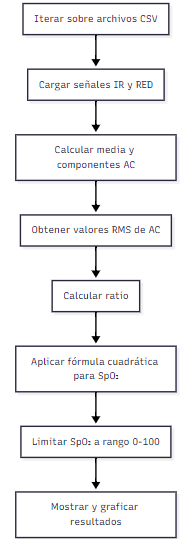
\includegraphics[width=0.25\linewidth]{img/SpO2_algo_v4.png}
    \caption{Diagrama de bloques del algoritmo de estimación de SpO$_2$ por Ratio y fórmula cuadrática. \textit{Elaboración propia.}}
    \label{fig: SpO2_algo_v4}
\end{figure}

\subsubsection{Algoritmo 2: mediante ratio AC/DC y modelo lineal calibrado}

El desarrollo de este algoritmo está implementado en el notebook \texttt{tabla\_LUT.ipynb}, cuyo funcionamiento se ilustra en la figura~\ref{fig:tabla_LUT2}.


\begin{figure}[H]
    \centering
    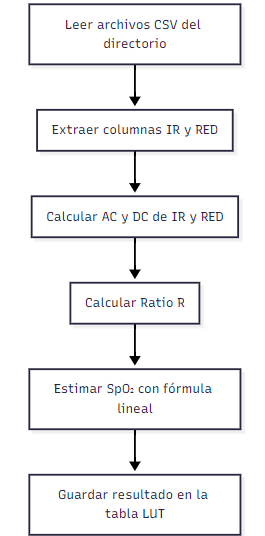
\includegraphics[width=0.25\linewidth]{img/tabla_LUT.png}
    \caption{Diagrama de bloques del algoritmo de estimación de SpO$_2$ por Ratio y modelo lineal. \textit{Elaboración propia.}}
    \label{fig:tabla_LUT2}
\end{figure}


\subsubsection{Algoritmo 3: Estimación por regresión lineal}

El algoritmo descrito puede consultarse en el notebook \texttt{Paper\_CS.ipynb}. Su flujo de ejecución se representa en la figura~\ref{fig: Paper_CS2}.

\begin{figure}[H]
    \centering
    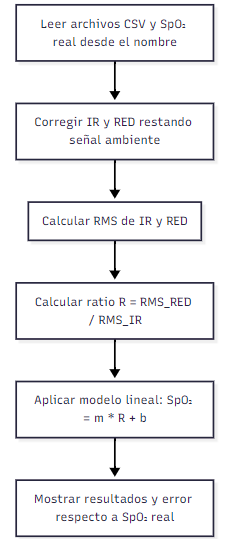
\includegraphics[scale=0.5]{img/Paper_CS.png}
    \caption{Diagrama de bloques del algoritmo de estimación de SpO$_2$ por regresión lineal.\textit{Elaboración propia.}}
    \label{fig: Paper_CS2}
\end{figure}

\subsubsection{Algoritmo 4: Estimación mediante tabla personalizada}

La implementación detallada de este algoritmo se encuentra en el notebook \texttt{uch\_spo2\_table.ipynb}. La figura~\ref{fig: uch_spo2_table2} muestra de forma esquemática su estructura y funcionamiento.

\begin{figure}[H]
    \centering
    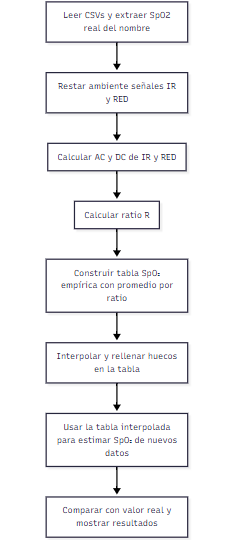
\includegraphics[scale =0.6]{img/uch_spo2_table.png}
    \caption{Diagrama de bloques del algoritmo de estimación de SpO$_2$ basado en tabla personalizada.\textit{Elaboración propia.}}
    \label{fig: uch_spo2_table2}
\end{figure}

\newpage

\subsection{Algoritmo final en el firmware}


\begin{figure}[H]
    \centering
    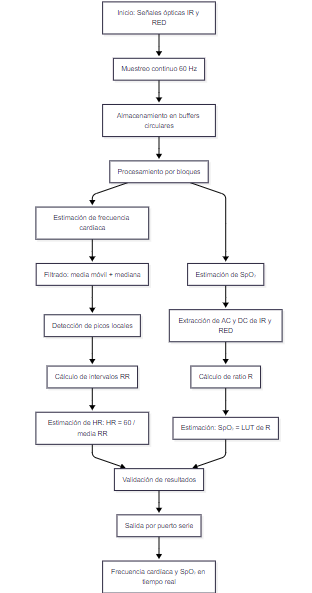
\includegraphics[width=0.75\linewidth]{img/flujo_firmware.png}
    \caption{Algoritmo de estimación de ambos parámetros en el propio firmware. El algoritmo ha sido explicado en la sección de metodología de la memoria.\textit{Elaboración propia.}}
    \label{fig:flujo_firmware}
\end{figure}